% ============================================================
%  PROTEA — Doctoral Thesis Defence (PhD)
%  Slide deck: ~30 slides, 50 min talk + 10 min Q&A
%  Author: Francisco Miguel Perez Canales
%  Co-supervisors: David Orellana-Martin + Ana M. Rojas
%  Universidad de Sevilla, Programa de Doctorado en Bioinformatica
% ============================================================
\documentclass[12pt, aspectratio=169]{beamer}

% ── Theme ───────────────────────────────────────────────────
\usetheme{Madrid}
\usecolortheme{default}

% ── Colour palette ──────────────────────────────────────────
\definecolor{proteagreen}{RGB}{38, 120, 78}
\definecolor{linkblue}{RGB}{0, 70, 140}
\definecolor{lightgray}{RGB}{240, 240, 240}

\setbeamercolor{palette primary}{bg=proteagreen, fg=white}
\setbeamercolor{palette secondary}{bg=proteagreen!80, fg=white}
\setbeamercolor{palette tertiary}{bg=proteagreen!60, fg=white}
\setbeamercolor{palette quaternary}{bg=proteagreen!40, fg=white}
\setbeamercolor{structure}{fg=proteagreen}
\setbeamercolor{block title}{bg=proteagreen, fg=white}
\setbeamercolor{block body}{bg=lightgray}
\setbeamercolor{alerted text}{fg=linkblue}
\setbeamercolor{frametitle}{bg=proteagreen, fg=white}

% ── Fonts and language ──────────────────────────────────────
\usepackage[utf8]{inputenc}
\usepackage[T1]{fontenc}
\usepackage[english]{babel}
\usepackage{lmodern}

% ── Math ────────────────────────────────────────────────────
\usepackage{amsmath, amssymb}

% ── Tables ──────────────────────────────────────────────────
\usepackage{booktabs}
\usepackage{multirow}
\usepackage{array}
\usepackage{colortbl}

% ── Graphics ────────────────────────────────────────────────
\usepackage{graphicx}
\usepackage{tikz}
\usetikzlibrary{positioning, arrows.meta, fit, shapes.geometric,
                calc, backgrounds, shadows.blur, decorations.pathreplacing}
\usepackage{pgfplots}
\pgfplotsset{compat=1.18}

% ── Utilities ───────────────────────────────────────────────
\usepackage{xcolor}
\usepackage{microtype}

% ── Beamer settings ─────────────────────────────────────────
\setbeamertemplate{navigation symbols}{}
\setbeamertemplate{footline}{%
  \leavevmode%
  \hbox{%
    \begin{beamercolorbox}[wd=.33\paperwidth, ht=2.25ex, dp=1ex, center]{author in head/foot}%
      \usebeamerfont{author in head/foot}F.M.\ P\'{e}rez Canales
    \end{beamercolorbox}%
    \begin{beamercolorbox}[wd=.34\paperwidth, ht=2.25ex, dp=1ex, center]{title in head/foot}%
      \usebeamerfont{title in head/foot}PROTEA Doctoral Defence
    \end{beamercolorbox}%
    \begin{beamercolorbox}[wd=.33\paperwidth, ht=2.25ex, dp=1ex, right]{date in head/foot}%
      \usebeamerfont{date in head/foot}\insertframenumber{}/\inserttotalframenumber\hspace*{2ex}
    \end{beamercolorbox}%
  }%
}

% ── Custom commands ─────────────────────────────────────────
\newcommand{\fmax}{$F_{\max}$}
\newcommand{\highlight}[1]{\textcolor{proteagreen}{\textbf{#1}}}
\newcommand{\todo}[1]{\textcolor{red}{\textbf{[TODO: #1]}}}

% ── Metadata ────────────────────────────────────────────────
\title[PROTEA -- Doctoral Defence]{%
  PROTEA: PROtein funcTional Embedding-based Annotation%
}
\subtitle{Doctoral Thesis Defence}
\author[F.M.\ P\'{e}rez Canales]{%
  Francisco Miguel P\'{e}rez Canales\\[4pt]
  {\small Co-supervisors: David Orellana-Mart\'{i}n \& Ana M.\ Rojas}%
}
\institute[Univ.\ Sevilla]{%
  Programa de Doctorado en Bioinform\'{a}tica\\
  Universidad de Sevilla%
}
\date{Academic Year 2025/2026}

% ============================================================
\begin{document}

% ── Slide 1: Title ──────────────────────────────────────────
\begin{frame}[plain]
  \titlepage
\end{frame}

% ── Slide 2: Outline ────────────────────────────────────────
\begin{frame}{Talk Overview}
  \begin{columns}[t]
    \column{0.48\textwidth}
      \textbf{Part I: Context and Motivation} \newline
      \begin{itemize}
        \item The annotation gap problem
        \item Gene Ontology and CAFA benchmarks
        \item The twilight zone of sequence identity
      \end{itemize}
      \vspace{1em}
      \textbf{Part II: PROTEA Platform}
      \begin{itemize}
        \item Design goals and architecture
        \item Plugin system and deployment
        \item Versioned data model
      \end{itemize}
    \column{0.48\textwidth}
      \textbf{Part III: Research Methods}
      \begin{itemize}
        \item PLM-KNN baseline
        \item Feature engineering (56 features)
        \item LightGBM re-ranker
      \end{itemize}
      \vspace{1em}
      \textbf{Part IV: Evaluation}
      \begin{itemize}
        \item Leakage-free temporal holdout
        \item NK/LK/PK results and ablation
        \item Comparison with external tools
        \item CAFA~6 team result
      \end{itemize}
  \end{columns}
  \vspace{0.5em}
  {\small \textbf{50 min talk + 10 min Q\&A} $\approx$ 30 slides}
\end{frame}

% ============================================================
%  PART I: Context and Motivation
% ============================================================

% ── Slide 3: The annotation gap ─────────────────────────────
\begin{frame}{The Protein Annotation Gap}
  \begin{columns}[c]
    \column{0.55\textwidth}
      \begin{block}{The Scale Problem}
        \begin{itemize}
          \item UniProt: \textbf{$>$250 million} sequences (early 2026)
          \item Experimentally annotated: \textbf{$<$0.02\,\%}
          \item Gap grows with every new sequencing campaign
          \item Under-studied organisms are disproportionately unannotated
        \end{itemize}
      \end{block}
      \vspace{0.5em}
      \begin{alertblock}{Consequence}
        Classical alignment (BLAST) breaks down below
        $\approx$30\,\% sequence identity -- the ``twilight zone''.
        Most evolutionary space is inaccessible.
      \end{alertblock}
    \column{0.40\textwidth}
      \centering
      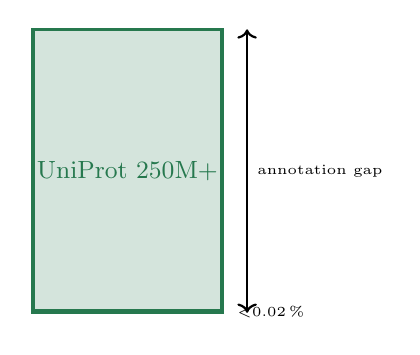
\begin{tikzpicture}[scale=0.8]
        \draw[proteagreen, very thick, fill=proteagreen!20]
              (0,0) rectangle (3, 4.5)
              node[midway, align=center, font=\small] {UniProt 250M+};
        \draw[proteagreen, very thick, fill=proteagreen]
              (0,0) rectangle (3, 0.04);
        \node[right, font=\tiny, xshift=2pt] at (3, 0.02) {$<$0.02\,\%};
        \draw[<->, thick] (3.4, 0) -- (3.4, 4.5)
              node[midway, right, font=\tiny, align=left] {annotation gap};
      \end{tikzpicture}
  \end{columns}
\end{frame}

% ── Slide 4: Gene Ontology ───────────────────────────────────
\begin{frame}{Gene Ontology and the CAFA Challenge}
  \begin{columns}[t]
    \column{0.48\textwidth}
      \textbf{Gene Ontology (GO)}
      \begin{itemize}
        \item Species-independent vocabulary for protein function
        \item Three aspects: \textbf{MFO}, \textbf{BPO}, \textbf{CCO}
        \item Directed acyclic graph (DAG) structure
        \item True-path rule: a specific term implies all ancestors
        \item Evidence codes: \texttt{EXP, IDA, IMP, IGI, IEP, IPI} (experimental)
      \end{itemize}
    \column{0.48\textwidth}
      \textbf{CAFA Benchmarks}
      \begin{itemize}
        \item Critical Assessment of protein Function Annotation
        \item International challenge since 2011
        \item Protocol: predict at $t_0$, evaluate against new annotations at $t_1$
        \item Metric: \fmax{} (max $F_1$ over confidence thresholds)
        \item IA-weighted: rare terms count more
      \end{itemize}
      \vspace{0.5em}
      \begin{block}{This thesis}
        Applies CAFA temporal protocol rigorously to all evaluation.
      \end{block}
  \end{columns}
\end{frame}

% ── Slide 5: PLMs and KNN ───────────────────────────────────
\begin{frame}{Protein Language Models and KNN Transfer}
  \begin{columns}[c]
    \column{0.55\textwidth}
      \textbf{Protein Language Models (PLMs)}
      \begin{itemize}
        \item Transformers trained on millions of protein sequences
        \item Masked-language objective learns structural/functional signal
        \item Examples: ESM-2, ESM-C, ProtT5, Ankh, ProstT5
        \item Single forward pass $\Rightarrow$ dense vector representation
      \end{itemize}
      \vspace{0.5em}
      \textbf{PLM-KNN Annotation Transfer}
      \begin{enumerate}
        \item Embed query + all Swiss-Prot reference sequences
        \item Retrieve $k$ nearest neighbours (cosine distance)
        \item Aggregate GO annotations from neighbours
        \item Output ranked GO term predictions
      \end{enumerate}
    \column{0.40\textwidth}
      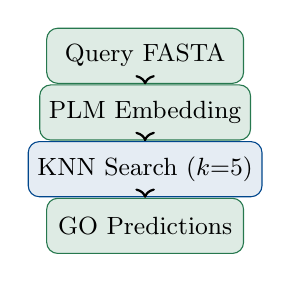
\begin{tikzpicture}[scale=0.72, font=\small]
        \node[draw=proteagreen, fill=proteagreen!15, rounded corners, align=center,
              minimum width=2.5cm, minimum height=0.7cm] (q) at (0,4)
              {Query FASTA};
        \node[draw=proteagreen, fill=proteagreen!15, rounded corners, align=center,
              minimum width=2.5cm, minimum height=0.7cm] (plm) at (0,3)
              {PLM Embedding};
        \node[draw=linkblue, fill=linkblue!10, rounded corners, align=center,
              minimum width=2.5cm, minimum height=0.7cm] (knn) at (0,2)
              {KNN Search ($k$=5)};
        \node[draw=proteagreen, fill=proteagreen!15, rounded corners, align=center,
              minimum width=2.5cm, minimum height=0.7cm] (go) at (0,1)
              {GO Predictions};
        \draw[->, thick] (q) -- (plm);
        \draw[->, thick] (plm) -- (knn);
        \draw[->, thick] (knn) -- (go);
      \end{tikzpicture}
  \end{columns}
\end{frame}

% ── Slide 6: Thesis Statement ────────────────────────────────
\begin{frame}{Thesis Statement and Research Questions}
  \begin{block}{Thesis Statement}
    PROTEA demonstrates that a contracts-first, plugin-driven platform for
    protein function annotation can simultaneously deliver a reproducible,
    leakage-free evaluation methodology, quantifiable gains from feature-engineered
    re-ranking over PLM-embedding baselines, and independently verifiable deployment
    as a public benchmark submission.
  \end{block}

  \vspace{0.8em}
  \textbf{Four Research Questions:}
  \begin{itemize}
    \item \textbf{RQ1:} Can PLM-KNN match or exceed alignment-based methods, and how does
               the answer change as PLMs evolve?
    \item \textbf{RQ2:} Do alignment statistics, taxonomy, and ontology-graph features
               provide complementary signal beyond the embedding baseline?
    \item \textbf{RQ3:} How can a reproducible pipeline be designed to run across
               development, cloud, HPC, and airgapped environments without code branching?
    \item \textbf{RQ4:} How can the ``why'' of a research platform be captured operationally
               for an auditable trace?
  \end{itemize}
\end{frame}

% ============================================================
%  PART II: PROTEA Platform
% ============================================================

% ── Slide 7: High-level Architecture ───────────────────────
\begin{frame}{PROTEA: High-Level Architecture}
  \begin{columns}[c]
    \column{0.55\textwidth}
      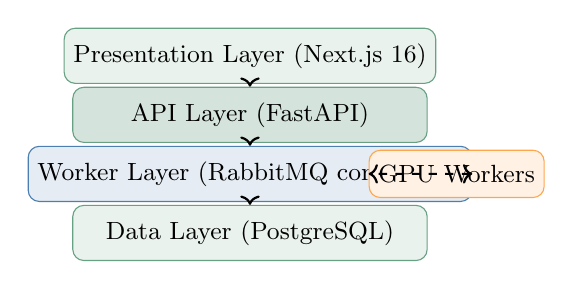
\begin{tikzpicture}[scale=0.75, font=\small]
        % Presentation
        \node[draw=proteagreen!70, fill=proteagreen!10, rounded corners,
              minimum width=4.5cm, minimum height=0.7cm, align=center] (ui)
              at (0,5) {Presentation Layer (Next.js 16)};
        % API
        \node[draw=proteagreen!70, fill=proteagreen!20, rounded corners,
              minimum width=4.5cm, minimum height=0.7cm, align=center] (api)
              at (0,4) {API Layer (FastAPI)};
        % Workers
        \node[draw=linkblue!70, fill=linkblue!10, rounded corners,
              minimum width=4.5cm, minimum height=0.7cm, align=center] (workers)
              at (0,3) {Worker Layer (RabbitMQ consumers)};
        % Data
        \node[draw=proteagreen!70, fill=proteagreen!10, rounded corners,
              minimum width=4.5cm, minimum height=0.7cm, align=center] (data)
              at (0,2) {Data Layer (PostgreSQL)};
        % GPU
        \node[draw=orange!70, fill=orange!10, rounded corners,
              minimum width=2cm, minimum height=0.6cm, align=center] (gpu)
              at (3.5,3) {GPU Workers};
        \draw[->, thick] (ui) -- (api);
        \draw[->, thick] (api) -- (workers);
        \draw[->, thick] (workers) -- (data);
        \draw[<->, thick, dashed] (workers) -- (gpu);
      \end{tikzpicture}
    \column{0.40\textwidth}
      \textbf{Key Properties}
      \begin{itemize}
        \item FastAPI + SQLAlchemy 2.0 + PostgreSQL 16
        \item RabbitMQ for task dispatch (10 queues)
        \item 33 registered operations
        \item Operation abstraction: every domain unit is testable and substitutable
        \item 17 REST API routers
        \item Reference set: \highlight{527,000} Swiss-Prot sequences
      \end{itemize}
  \end{columns}
\end{frame}

% ── Slide 8: Plugin Architecture ─────────────────────────────
\begin{frame}{Plugin Architecture: Seven Repositories}
  \begin{columns}[c]
    \column{0.54\textwidth}
      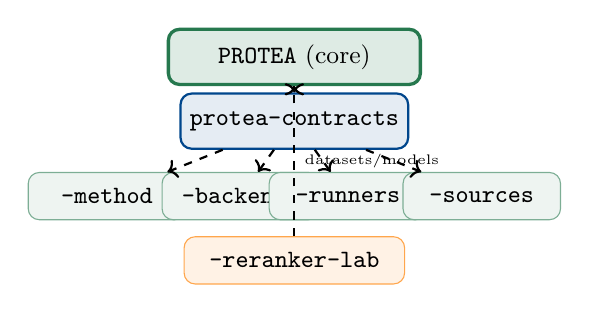
\begin{tikzpicture}[scale=0.68, font=\small]
        \node[draw=proteagreen, very thick, fill=proteagreen!15, rounded corners,
              minimum width=3.2cm, minimum height=0.7cm, align=center] (core)
              at (0,4) {\texttt{PROTEA} (core)};
        \node[draw=linkblue, thick, fill=linkblue!10, rounded corners,
              minimum width=2.8cm, minimum height=0.7cm, align=center] (contracts)
              at (0,2.8) {\texttt{protea-contracts}};
        \node[draw=proteagreen!60, fill=proteagreen!8, rounded corners,
              minimum width=2.0cm, minimum height=0.6cm, align=center] (method)
              at (-3.5, 1.4) {\texttt{-method}};
        \node[draw=proteagreen!60, fill=proteagreen!8, rounded corners,
              minimum width=2.0cm, minimum height=0.6cm, align=center] (backends)
              at (-1.0, 1.4) {\texttt{-backends}};
        \node[draw=proteagreen!60, fill=proteagreen!8, rounded corners,
              minimum width=2.0cm, minimum height=0.6cm, align=center] (runners)
              at (1.0, 1.4) {\texttt{-runners}};
        \node[draw=proteagreen!60, fill=proteagreen!8, rounded corners,
              minimum width=2.0cm, minimum height=0.6cm, align=center] (sources)
              at (3.5, 1.4) {\texttt{-sources}};
        \node[draw=orange!70, fill=orange!10, rounded corners,
              minimum width=2.8cm, minimum height=0.6cm, align=center] (lab)
              at (0, 0.2) {\texttt{-reranker-lab}};
        \draw[->, thick] (core) -- (contracts);
        \draw[->, thick, dashed] (contracts) -- (method);
        \draw[->, thick, dashed] (contracts) -- (backends);
        \draw[->, thick, dashed] (contracts) -- (runners);
        \draw[->, thick, dashed] (contracts) -- (sources);
        \draw[->, thick, dashed] (lab) -- (core)
              node[midway, right, font=\tiny] {datasets/models};
      \end{tikzpicture}
    \column{0.42\textwidth}
      \textbf{Plugin details:}
      \begin{itemize}
        \item \texttt{-method}: LAFA inference layer
        \item \texttt{-backends}: 8 PLM adapters (ESM-2/C, ProtT5, Ankh, ProstT5)
        \item \texttt{-runners}: LightGBM training runner
        \item \texttt{-sources}: GOA, QuickGO annotation loaders
        \item \texttt{-reranker-lab}: offline training (consumes frozen datasets)
      \end{itemize}
      \vspace{0.3em}
      Discovery via Python \texttt{entry\_points}.
      New PLM = one class implementing \texttt{EmbeddingBackend} ABC.
  \end{columns}
\end{frame}

% ── Slide 9: Versioned Data Model ────────────────────────────
\begin{frame}{Versioned Data Model and Reproducibility}
  \begin{columns}[t]
    \column{0.52\textwidth}
      \textbf{Every prediction is permanently linked to:}
      \begin{itemize}
        \item \texttt{EmbeddingConfig} UUID (PLM + pooling strategy)
        \item \texttt{AnnotationSet} (GOA release number)
        \item \texttt{OntologySnapshot} (OBO release date)
        \item \texttt{Dataset} snapshot with schema fingerprint
        \item \texttt{RerankerModel} (LightGBM booster + feature hash)
        \item \texttt{ExperimentRun} + \texttt{Job.findings} narrative
      \end{itemize}
      \vspace{0.5em}
      \begin{block}{Reproducibility guarantee}
        Re-running the same \texttt{train\_reranker\_auto} payload
        against the same DB state produces \emph{identical} models
        and results. New GOA release: extend version list, shift
        test window.
      \end{block}
    \column{0.44\textwidth}
      \textbf{31 Architecture Decision Records (D1--D31)}
      \begin{itemize}
        \item Every non-obvious choice is recorded with its rationale
        \item Examples: plugin split (D1), pgvector for storage only (D5),
              NumPy/FAISS for search (D8), contracts-first (D15)
      \end{itemize}
      \vspace{0.3em}
      \textbf{Observability}
      \begin{itemize}
        \item OpenTelemetry SDK layer
        \item 5 Grafana dashboards (API latency, queue depth, worker throughput)
        \item \texttt{JobEvent} audit trail per run
      \end{itemize}
  \end{columns}
\end{frame}

% ── Slide 10: Deployment Matrix ──────────────────────────────
\begin{frame}{Multi-Environment Deployment}
  \begin{center}
    \begin{tabular}{lll}
      \toprule
      \textbf{Environment} & \textbf{Mechanism} & \textbf{Validation} \\
      \midrule
      Development   & \texttt{docker compose} & CI + end-to-end (T-OPS.11) \\
      Cloud         & Helm chart (Kubernetes)  & Deploy test gates each release \\
      Cloud (swarm) & Docker Swarm stack       & \texttt{docker stack deploy} \\
      HPC           & SLURM \texttt{sbatch} templates & Apptainer-compatible \\
      \midrule
      \multicolumn{3}{l}{\textbf{LAFA submissions: same codebase, no code branching}} \\
      \midrule
      LAFA KNN-v1   & Container image (GHCR)   & Published, independently verifiable \\
      LAFA 8-PLM    & Container image (GHCR)   & Ensemble container \\
      LAFA protea-v18 & Container image (GHCR) & Full pipeline (PR \#305) \\
      \bottomrule
    \end{tabular}
  \end{center}
  \vspace{0.5em}
  {\small The contracts-first split (ADR D15) means \texttt{protea-method} has no FastAPI or ORM dependencies; it runs standalone from \texttt{pip install protea-method}.}
\end{frame}

% ============================================================
%  PART III: Research Methods
% ============================================================

% ── Slide 11: Evaluation Protocol Overview ──────────────────
\begin{frame}{Evaluation Protocol: Leakage-Free Temporal Holdout}
  \begin{columns}[c]
    \column{0.55\textwidth}
      \textbf{15 GOA Swiss-Prot snapshots (releases 160--229)}
      \begin{itemize}
        \item Evidence codes: EXP, IDA, IMP, IGI, IEP, IPI
        \item Training for re-ranker: releases 160--215 (12 splits)
        \item Primary reference $t_0$: release 220
        \item Primary test $t_1$: release 229 (or 230)
      \end{itemize}
      \vspace{0.5em}
      \begin{alertblock}{Why leakage-free matters}
        Training and evaluating on the same annotation snapshot inflates
        \fmax. The leakage-free protocol isolates genuine generalisation.
        Leakage-corrupted numbers are substantially higher.
      \end{alertblock}
    \column{0.40\textwidth}
      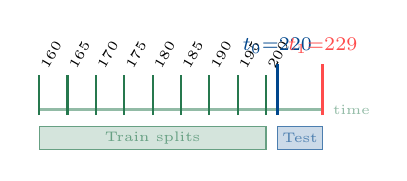
\begin{tikzpicture}[scale=0.72, font=\small]
        \draw[proteagreen!50, thick] (0,0) -- (5,0)
              node[right, font=\tiny] {time};
        % splits
        \foreach \x/\lbl in {0/160, 0.5/165, 1/170, 1.5/175, 2/180,
                              2.5/185, 3/190, 3.5/195, 4/200} {
          \draw[proteagreen, thick] (\x, -0.1) -- (\x, 0.6);
          \node[font=\tiny, rotate=60, anchor=west] at (\x, 0.6) {\lbl};
        }
        % t0 t1
        \draw[linkblue, very thick] (4.2, -0.1) -- (4.2, 0.8)
              node[above, font=\scriptsize] {$t_0$=220};
        \draw[red!70, very thick] (5.0, -0.1) -- (5.0, 0.8)
              node[above, font=\scriptsize] {$t_1$=229};
        \draw[proteagreen!70, fill=proteagreen!20]
              (0, -0.7) rectangle (4.0, -0.3)
              node[midway, font=\tiny] {Train splits};
        \draw[linkblue!70, fill=linkblue!20]
              (4.2, -0.7) rectangle (5.0, -0.3)
              node[midway, font=\tiny] {Test};
      \end{tikzpicture}
      \vspace{0.5em}
      {\small Metric: \fmax{} with IA weighting (\texttt{IA\_cafa6.tsv})}
  \end{columns}
\end{frame}

% ── Slide 12: Evaluation Categories NK/LK/PK ────────────────
\begin{frame}{Evaluation Categories: NK / LK / PK}
  \begin{columns}[t]
    \column{0.32\textwidth}
      \begin{block}{NK: No-Knowledge}
        Protein had \emph{no} experimental annotations in any namespace at $t_0$.
        All new annotations across all namespaces form the ground truth.
        \vspace{0.2em}

        \textit{Most challenging: entering the experimental literature for the first time.}
      \end{block}
    \column{0.32\textwidth}
      \begin{block}{LK: Limited-Knowledge}
        Protein had annotations in some namespaces at $t_0$, but \emph{not} in
        namespace $S$. New annotations in $S$ at $t_1$ are the ground truth.
        \vspace{0.2em}

        \textit{Intermediate difficulty: cross-aspect transfer.}
      \end{block}
    \column{0.32\textwidth}
      \begin{block}{PK: Partial-Knowledge}
        Protein already had annotations in namespace $S$ at $t_0$ and gained
        additional annotations. Only novel terms are ground truth; known terms
        passed as exclusion set.
        \vspace{0.2em}

        \textit{Hardest to improve over baseline: model already knows some function.}
      \end{block}
  \end{columns}
  \vspace{1em}
  \begin{center}
    \begin{tabular}{lrr}
      \toprule
      Category & Proteins & Annotations (GOA 220$\to$229 delta) \\
      \midrule
      NK & 2,831 & 6,953 \\
      LK & 3,410 & 5,520 \\
      PK & 15,313 & 27,541 \\
      \midrule
      \textbf{Total} & \textbf{20,281} & \textbf{40,014} \\
      \bottomrule
    \end{tabular}
  \end{center}
\end{frame}

% ── Slide 13: Baseline -- KNN ────────────────────────────────
\begin{frame}{Experiment 1--2: PLM-KNN Baseline}
  \begin{columns}[t]
    \column{0.48\textwidth}
      \textbf{Experiment 1: Effect of $k$}
      \begin{itemize}
        \item Tested $k \in \{5, 10, 20, 50\}$
        \item \highlight{$k = 5$ optimal} across all categories/aspects
        \item Performance degrades monotonically with larger $k$
        \item Functional signal concentrated in nearest neighbours
      \end{itemize}
      \vspace{0.5em}
      \begin{tabular}{lccc}
        \toprule
        $k$ & NK-MFO & LK-MFO & NK-CCO \\
        \midrule
        \textbf{5}  & \textbf{0.590} & \textbf{0.558} & \textbf{0.668} \\
        10 & 0.574 & 0.537 & 0.656 \\
        20 & 0.564 & 0.528 & 0.649 \\
        \bottomrule
      \end{tabular}
    \column{0.48\textwidth}
      \textbf{Experiment 2: Aspect-Separated vs Unified KNN}
      \begin{itemize}
        \item Separated: one index per GO namespace
        \item Unified: single index, all namespaces
        \item Difference $\leq 0.011$ in all cells
        \item Retain \texttt{aspect\_separated=true}: uniform coverage
      \end{itemize}
      \vspace{0.5em}
      \textbf{Experiment 3: Heuristic Scoring}
      \begin{itemize}
        \item Alignment-weighted: emb=0.5 + NW=0.3 + SW=0.2
        \item \highlight{+1.5 to 4\%} \fmax{} over embedding-only
        \item Confirms alignment and embeddings are complementary
      \end{itemize}
  \end{columns}
\end{frame}

% ── Slide 14: Feature Engineering ───────────────────────────
\begin{frame}{Feature Engineering: 56-Feature Registry}
  \begin{columns}[t]
    \column{0.52\textwidth}
      \textbf{Feature Families (56 total)}
      \begin{itemize}
        \item[\textbullet] \textbf{Embedding:} Cosine distance (PLM-derived)
        \item[\textbullet] \textbf{Alignment:} NW + SW identity/score (BLOSUM62)
        \item[\textbullet] \textbf{Taxonomy:} NCBI taxonomy distance (ete3)
        \item[\textbullet] \textbf{Aggregation:} Vote fraction, GO term frequency
        \item[\textbullet] \textbf{anc2vec-q:} GO-graph embeddings vs query's known terms
        \item[\textbullet] \textbf{anc2vec-nbr:} Candidate GO term in ontology space
        \item[\textbullet] \textbf{PCA:} Per-PLM PCA(16) projection
        \item[\textbullet] \textbf{Lineage:} Ancestor/descendant-of-known flags (T-RES.1b)
        \item[\textbullet] \textbf{GO context:} Term depth, evidence code
      \end{itemize}
    \column{0.44\textwidth}
      \textbf{Schema fingerprint}
      \begin{itemize}
        \item Feature registry hashed at training time
        \item Stored \texttt{RerankerModel} auto-invalidated on schema change
        \item Prevents silent mismatches between train and inference
      \end{itemize}
      \vspace{0.5em}
      \begin{block}{From 52 to 56 features}
        T-RES.1b (PR \#304) added four lineage features:
        \texttt{lineage\_is\_ancestor\_of\_known},
        \texttt{lineage\_is\_descendant\_of\_known},
        \texttt{lineage\_ancestor\_of\_count},
        \texttt{lineage\_descendant\_of\_count}
      \end{block}
  \end{columns}
\end{frame}

% ── Slide 15: Re-Ranker Evolution ────────────────────────────
\begin{frame}{LightGBM Re-Ranker: Evolution v1 to v3}
  \begin{columns}[t]
    \column{0.50\textwidth}
      \textbf{v1 (Exp.~4): Per-Aspect Models}
      \begin{itemize}
        \item 9 models: NK/LK/PK $\times$ BPO/MFO/CCO
        \item Problem: extreme class imbalance ($<$0.2\%)
        \item 6/9 models stop at iteration 1
        \item CCO improves, MFO \emph{degrades} vs heuristic
      \end{itemize}
      \vspace{0.5em}
      \textbf{v2 (Exp.~5): Per-Category + IA Weighting}
      \begin{itemize}
        \item 3 models: NK, LK, PK (3$\times$ more training data)
        \item IA-weighted loss aligns with evaluation metric
        \item More stable; MFO collapse fixed
        \item But: alignment/taxonomy were NULL during training!
      \end{itemize}
    \column{0.46\textwidth}
      \textbf{v3 (Exp.~6): Full Feature Set, Leakage-Free}
      \begin{itemize}
        \item Full 52-feature schema (NW, SW, taxonomy, anc2vec)
        \item Leakage-free dataset \texttt{bench-v1-K5-filtered}
        \item GOA~220$\to$230 eval split
        \item 3 seeds ($\sigma \leq 0.003$)
      \end{itemize}
      \vspace{0.3em}
      \begin{alertblock}{Key result}
        NK-BPO: $0.412 \to 0.599$ (+0.187)\\
        NK-MFO: $0.590 \to 0.646$ (+0.056)\\
        LK-BPO: $0.467 \to 0.620$ (+0.153)
      \end{alertblock}
  \end{columns}
\end{frame}

% ============================================================
%  PART IV: Evaluation
% ============================================================

% ── Slide 16: Full Results Table (v3) ───────────────────────
\begin{frame}{Experiment 6: Re-Ranker v3 Full Results}
  \begin{center}
    \begin{tabular}{l ccc ccc ccc}
      \toprule
      & \multicolumn{3}{c}{\textbf{NK}} & \multicolumn{3}{c}{\textbf{LK}} & \multicolumn{3}{c}{\textbf{PK}} \\
      \cmidrule(lr){2-4} \cmidrule(lr){5-7} \cmidrule(lr){8-10}
      \textbf{Method} & BPO & MFO & CCO & BPO & MFO & CCO & BPO & MFO & CCO \\
      \midrule
      Baseline (emb.~only)$^\dagger$ & 0.412 & 0.590 & 0.668 & 0.467 & 0.558 & 0.675 & 0.187 & 0.278 & 0.325 \\
      Alignment weighted$^\dagger$    & 0.428 & 0.611 & 0.683 & 0.500 & 0.598 & 0.699 & 0.201 & 0.285 & 0.337 \\
      Re-ranker v2$^\dagger$          & 0.425 & 0.607 & 0.689 & 0.486 & 0.575 & 0.707 & 0.199 & 0.297 & 0.335 \\
      \rowcolor{proteagreen!15}
      \textbf{Re-ranker v3} & \textbf{0.599} & \textbf{0.646} & \textbf{0.775} & \textbf{0.620} & \textbf{0.606} & \textbf{0.794} & 0.165 & 0.293 & 0.346 \\
      \bottomrule
    \end{tabular}
  \end{center}
  \vspace{0.3em}
  {\small $^\dagger$ Pre-leakage-fix dataset (22-feature schema, GOA 220$\to$229); not directly comparable with v3 row.}
  \vspace{0.3em}
  \begin{itemize}
    \item v3 shows large NK and LK gains (leakage-free, full feature set)
    \item PK-BPO lower in v3: leakage-fix tightens PK positive criterion
  \end{itemize}
\end{frame}

% ── Slide 17: v9 Study and cafaeval ─────────────────────────
\begin{frame}{Experiment 8: Re-Ranker v9 Study and cafaeval Validation}
  \begin{columns}[t]
    \column{0.50\textwidth}
      \textbf{Study v9 (2026-05-01): 56-feature schema}
      \begin{itemize}
        \item 3-seed replication (42, 7, 137); std $\leq 0.003$
        \item Validated with \texttt{cafaeval} (prop=fill, norm=cafa)
        \item Lab metric: avg \fmax = \highlight{0.2881} (9 cells)
        \item cafaeval avg: \highlight{0.5427} (CAFA-comparable)
      \end{itemize}
      \vspace{0.4em}
      \textbf{Why the gap (lab vs cafaeval)?}
      \begin{itemize}
        \item cafaeval propagates predictions through GO DAG
        \item Specific predictions gain ancestors for free
        \item Most impactful for PK-MFO (4.1$\times$ ratio)
      \end{itemize}
    \column{0.46\textwidth}
      \textbf{Selected cafaeval \fmax (v9):}
      \vspace{0.3em}
      \begin{tabular}{lrr}
        \toprule
        Cell & Lab & Cafaeval \\
        \midrule
        NK-BPO & 0.4649 & 0.5238 \\
        NK-MFO & 0.4605 & 0.6833 \\
        NK-CCO & 0.4840 & 0.7383 \\
        LK-BPO & 0.3570 & 0.5542 \\
        LK-MFO & 0.2440 & 0.6265 \\
        \midrule
        Avg (9 cells) & 0.2899 & \textbf{0.5427} \\
        \bottomrule
      \end{tabular}
      \vspace{0.3em}
      {\small v9 vs KNN baseline: all 9 cells $p < 0.0001$ (paired bootstrap, 2000 resamples).}
  \end{columns}
\end{frame}

% ── Slide 18: Feature Importance ─────────────────────────────
\begin{frame}{Feature Importance Analysis (v3/v9)}
  \begin{columns}[t]
    \column{0.50\textwidth}
      \textbf{Top features by LightGBM gain (v3, seed 42)}
      \begin{itemize}
        \item \highlight{\texttt{nb\_vote\_frac}}: top in NK and LK
        \item \highlight{\texttt{go\_term\_freq}}: top in PK
        \item \highlight{\texttt{anc2vec\_n\_cos}} and \texttt{anc2vec\_q\_maxcos}: top-10 in all categories
        \item Raw embedding distance: \emph{not in top-10 for any category}
      \end{itemize}
      \vspace{0.5em}
      \textbf{Key insight:} Re-ranker uses embedding primarily as a candidate-generation
      filter, not as a final ranking signal.
    \column{0.46\textwidth}
      \textbf{Leave-one-family-out ablation (v9, 3 cells)}
      \vspace{0.3em}
      \begin{tabular}{lr}
        \toprule
        Family & Mean $\Delta F_{\max}$ \\
        \midrule
        \texttt{anc2vec\_query} & \highlight{+0.1449} \\
        \texttt{knn} & +0.0101 \\
        \texttt{knn\_vote} & +0.0046 \\
        \texttt{knn\_distance} & +0.0018 \\
        \texttt{alignment\_nw} & +0.0002 \\
        \texttt{taxonomy\_pair} & +0.0000 \\
        \bottomrule
      \end{tabular}
      \vspace{0.3em}
      {\small NK-BPO alone: \texttt{anc2vec\_query} $\Delta = +0.2565$.}
      Ontology-derived embeddings are the \emph{decisive} marginal signal.
  \end{columns}
\end{frame}

% ── Slide 19: Comparison with eggNOG-mapper ─────────────────
\begin{frame}{Experiment 7: Comparison with eggNOG-mapper}
  \begin{columns}[c]
    \column{0.55\textwidth}
      \begin{tabular}{l ccc ccc}
        \toprule
        & \multicolumn{3}{c}{\textbf{NK}} & \multicolumn{3}{c}{\textbf{LK}} \\
        \cmidrule(lr){2-4} \cmidrule(lr){5-7}
        \textbf{Method} & BPO & MFO & CCO & BPO & MFO & CCO \\
        \midrule
        eggNOG-m.$^\ddagger$ & 0.247 & 0.359 & 0.386 & 0.382 & 0.334 & 0.450 \\
        PROTEA base.$^\dagger$ & 0.412 & 0.590 & 0.668 & 0.467 & 0.558 & 0.675 \\
        \rowcolor{proteagreen!15}
        \textbf{v3} & \textbf{0.599} & \textbf{0.646} & \textbf{0.775} & \textbf{0.620} & \textbf{0.606} & \textbf{0.794} \\
        \bottomrule
      \end{tabular}
      \vspace{0.3em}
      {\small $^\dagger$~pre-leakage-fix; $^\ddagger$~eggNOG-mapper v2.1.13, DIAMOND + \texttt{--go\_evidence experimental}.}
    \column{0.40\textwidth}
      \textbf{Findings:}
      \begin{itemize}
        \item PROTEA baseline surpasses eggNOG-mapper in \highlight{8/9 cells}
        \item Absolute improvements up to +0.306 \fmax{} (NK-CCO)
        \item eggNOG-mapper coverage: 85.5\% (17,334/20,281 proteins)
        \item PLM embeddings outperform DIAMOND-based orthology transfer for NK and LK
      \end{itemize}
      \vspace{0.3em}
      {\small Caveats: different eval sets; eggNOG assigns uniform confidence; eggNOG DB v5.0.2 predates eval window.}
  \end{columns}
\end{frame}

% ── Slide 20: LB.2 / LB.3 Leakage-Fixed Champion ───────────
\begin{frame}{Leakage-Fixed Champion: v27-binary Multiseed (LB.2/LB.3)}
  \begin{columns}[c]
    \column{0.55\textwidth}
      \textbf{v27-binary recipe (anc2vec retrofix)}
      \begin{itemize}
        \item 3 seeds $\times$ 6 cells (NK+LK only)
        \item Selective avg: \highlight{0.6215 $\pm$ 0.0014} on v226
        \item Selective deploy: NK+LK $\to$ v27-binary, PK $\to$ KNN baseline
      \end{itemize}
      \vspace{0.5em}
      \textbf{Paired bootstrap CI (N=10,000, bench-v1-K5-v226-lineage)}
      \begin{itemize}
        \item 6/6 NK+LK CIs strictly positive at 95\%
        \item PK: policy-zero (KNN baseline wins)
        \item Publishable statistical claim for Chapter 6
      \end{itemize}
    \column{0.40\textwidth}
      \textbf{Feature importance (9 aspect-stable features):}
      \begin{itemize}
        \item Alignment + taxonomy family: score 0 gain
        \item NK+LK dominated by \texttt{anc2vec} + vote aggregation
        \item PK lineage-dominated (motivates selective deploy)
      \end{itemize}
      \vspace{0.3em}
      \begin{block}{Note: Multi-PLM sweep (FARM-EXP.13-18)}
        Full (PLM $\times$ K $\times$ recipe) grid on v226$\to$v230 in progress.
        \todo{Update with final FARM-EXP.13 grid when available}
      \end{block}
  \end{columns}
\end{frame}

% ── Slide 21: CAFA 6 Result ──────────────────────────────────
\begin{frame}{CAFA~6: Team Achievement}
  \begin{columns}[c]
    \column{0.55\textwidth}
      \begin{block}{CAFA~6 TEAM result}
        \begin{itemize}
          \item \highlight{2nd place} in the international CAFA~6 challenge
          \item This is a \textbf{team result}, not an individual submission
          \item The author was the technical motor of the submission
          \item PROTEA provided the platform and evaluation infrastructure
        \end{itemize}
      \end{block}
      \vspace{0.5em}
      \textbf{LAFA submissions (independently verifiable)}
      \begin{itemize}
        \item Three pre-built containers published to GHCR
        \item Same code path: development workstation $\to$ benchmark container
        \item No code branching required
      \end{itemize}
    \column{0.40\textwidth}
      \textbf{PROTEA as post-CAFA productisation}
      \begin{itemize}
        \item CAFA \#2 belongs to the research
        \item PROTEA is the platform enabling this and future work
        \item The pipeline is designed to be re-evaluable as new PLMs and GOA releases arrive
      \end{itemize}
      \vspace{0.5em}
      \todo{Confirm CAFA 6 team ranking number/citation with supervisors before defence}
  \end{columns}
\end{frame}

% ── Slide 22: 8-PLM Benchmark ───────────────────────────────
\begin{frame}{8-PLM Backend Benchmark}
  \begin{columns}[t]
    \column{0.52\textwidth}
      \textbf{PLM backends evaluated:}
      \begin{itemize}
        \item ESM-2 (150M, 650M, 3B parameters)
        \item ESM-C (300M, 600M)
        \item ProstT5
        \item ProtT5
        \item Ankh (base, large)
      \end{itemize}
      \vspace{0.3em}
      \textbf{Common evaluation surface:}
      \begin{itemize}
        \item bench-v1-K5-v226-lineage-\{plm\}
        \item $K \in \{3, 5, 10\}$
        \item v27-binary recipe per PLM
        \item \texttt{allplm}: derived multi-manifest trainer
      \end{itemize}
    \column{0.44\textwidth}
      \begin{block}{Hybrid-picker ceiling}
        Routing each query to the optimal backend per category-aspect cell:
        \highlight{0.4400 \fmax} (lab internal, 2026-04-20).
        Setting concrete target for future ensemble work.
      \end{block}
      \vspace{0.5em}
      \begin{alertblock}{FARM-EXP.13 in progress}
        Full (PLM $\times$ K $\times$ recipe) cafaeval grid on v226$\to$v230.
        \todo{Replace placeholder with final grid numbers when FARM-EXP.13 completes}
      \end{alertblock}
  \end{columns}
\end{frame}

% ── Slide 23: Contributions Summary ─────────────────────────
\begin{frame}{Summary of Contributions}
  \begin{columns}[t]
    \column{0.48\textwidth}
      \textbf{Platform}
      \begin{itemize}
        \item PROTEA: open-source distributed annotation platform
        \item Plugin architecture (7 repos, Python \texttt{entry\_points})
        \item Versioned relational data model (Alembic, full provenance)
        \item Multi-environment deployment (dev / cloud / HPC / airgapped)
        \item 31 Architecture Decision Records (D1--D31)
        \item OpenTelemetry observability layer
      \end{itemize}
      \vspace{0.3em}
      \textbf{Infrastructure}
      \begin{itemize}
        \item 33-operation catalogue
        \item 17 REST API routers
        \item \texttt{cafaeval-protea} fork (maintained)
        \item 3 LAFA container submissions
      \end{itemize}
    \column{0.48\textwidth}
      \textbf{Research Methods}
      \begin{itemize}
        \item 56-feature engineering registry with schema fingerprint
        \item Selective LightGBM re-ranker (per category + per aspect)
        \item Leakage-free temporal holdout (12 GOA splits for training)
        \item Gated-attention MIL head (opt-in, \texttt{protea-method})
      \end{itemize}
      \vspace{0.3em}
      \textbf{Empirical Results}
      \begin{itemize}
        \item NK-BPO $F_{\max}$: $0.412 \to 0.599$ (+0.187, leakage-free)
        \item v9 cafaeval avg \fmax: \highlight{0.5427}
        \item Outperforms eggNOG-mapper in 8/9 cells
        \item v27-binary selective: \highlight{0.6215 $\pm$ 0.0014}
        \item CAFA~6 \#2 (team result)
        \item Bootstrap CI: 6/6 NK+LK cells significant at 95\%
      \end{itemize}
  \end{columns}
\end{frame}

% ── Slide 24: Addressing Research Questions ─────────────────
\begin{frame}{Answers to the Research Questions}
  \begin{itemize}
    \item \textbf{RQ1 (PLM-KNN vs alignment):} Baseline surpasses eggNOG-mapper
          (DIAMOND-based) in 8/9 cells. Alignment features give +1.5 to 4\% \fmax.
          v9 cafaeval avg 0.5427 vs historical ceiling 0.4400.
          Plugin architecture allows re-evaluation as PLMs evolve.

    \item \textbf{RQ2 (Complementary features):} Yes. \texttt{anc2vec\_query}
          family alone contributes mean $\Delta F_{\max} = +0.1449$ (leave-one-out ablation).
          Alignment/taxonomy marginal ($\pm 0.01$). Feature engineering remains valuable.

    \item \textbf{RQ3 (Reproducible, scalable pipeline):} Versioned data model
          (EmbeddingConfig UUID + AnnotationSet + OntologySnapshot). Same payload reproduces
          identical models. Four deployment modes without code branching.
          Validated by LAFA container submissions.

    \item \textbf{RQ4 (Operational narrative):} \texttt{Job.findings} narrative
          model + \texttt{ExperimentRun} + 31 ADRs (D1--D31). Audit trace is integral
          to the platform, not a post-hoc add-on.
  \end{itemize}
\end{frame}

% ── Slide 25: Limitations ────────────────────────────────────
\begin{frame}{Limitations}
  \begin{columns}[t]
    \column{0.48\textwidth}
      \textbf{Evaluation scope}
      \begin{itemize}
        \item Single workstation (16 GB GPU). No multi-GPU/distributed training
        \item Comparison limited to eggNOG-mapper (BLAST, InterProScan pending)
        \item Temporal holdout does not fully eliminate high-identity leakage
        \item IA file (\texttt{IA\_cafa6.tsv}) computed for CAFA6; may not perfectly reflect specific GOA snapshots
      \end{itemize}
      \vspace{0.5em}
      \textbf{Model}
      \begin{itemize}
        \item Main experiments: ESMC 300M only
        \item Full 8-PLM benchmark cafaeval grid (FARM-EXP.13-18) in progress
        \item Hyperparameter sensitivity: 0.0283 spread on NK-BPO; per-cell tuning warranted
      \end{itemize}
    \column{0.48\textwidth}
      \textbf{Architecture}
      \begin{itemize}
        \item No structural information (AlphaFold/Foldseek) integrated
        \item Deep observability (T5.1b \texttt{traceparent}) still in review
        \item Benchmark may over-represent easily-annotated proteins
      \end{itemize}
      \vspace{0.5em}
      \textbf{Re-ranker}
      \begin{itemize}
        \item LK-BPO consistently favours heuristic over re-ranker in some configurations
        \item PK benefits less; selective-deploy policy partially addresses this
        \item Leakage-free ablation of v2 vs v3 pending (lab-runner LB.2)
      \end{itemize}
  \end{columns}
\end{frame}

% ── Slide 26: Future Work ────────────────────────────────────
\begin{frame}{Future Work}
  \begin{columns}[t]
    \column{0.48\textwidth}
      \textbf{Short-term}
      \begin{itemize}
        \item Complete FARM-EXP.13-18 grid (full PLM $\times$ K $\times$ recipe)
        \item Leakage-free ablation v2 vs v3 (lab-runner LB.2)
        \item Extended external comparison (BLAST, InterProScan under same temporal protocol)
        \item Ship T5.1b observability (end-to-end \texttt{traceparent})
      \end{itemize}
    \column{0.48\textwidth}
      \textbf{Research directions}
      \begin{itemize}
        \item Backend ensemble: meta-classifier over 8 PLMs (target: beat 0.4400 ceiling)
        \item MIL head ablation (gated-attention vs mean pooling across NK/LK/PK)
        \item Structure-aware embeddings (ESM-IF, Foldseek)
        \item Active learning: prioritise high-uncertainty proteins for experimental characterisation
        \item Ontology-aware scoring (hierarchical classifier, IC-weighted majority vote)
      \end{itemize}
  \end{columns}
\end{frame}

% ── Slide 27: Conclusions ────────────────────────────────────
\begin{frame}{Conclusions}
  \begin{block}{What was built}
    PROTEA is a contracts-first, plugin-driven, open-source distributed platform for
    scalable and reproducible protein function annotation using Gene Ontology terms.
    Seven repositories. 33 operations. 31 ADRs. Full provenance trail.
  \end{block}
  \vspace{0.5em}
  \begin{block}{What was demonstrated}
    \begin{itemize}
      \item PLM-KNN outperforms DIAMOND-based alignment transfer (8/9 cells vs eggNOG-mapper)
      \item Feature engineering raises NK-BPO \fmax{} by +0.187 over the embedding baseline
      \item \texttt{anc2vec\_query} (GO ancestry embeddings) is the decisive marginal signal
      \item Leakage-free evaluation reveals that leakage-corrupted numbers are substantially inflated
      \item Selective deploy (NK+LK: v27-binary; PK: KNN) gives 0.6215 $\pm$ 0.0014
      \item Same codebase deploys: workstation $\to$ docker compose $\to$ Kubernetes $\to$ HPC $\to$ LAFA container
    \end{itemize}
  \end{block}
  \vspace{0.3em}
  {\small PROTEA: \url{https://github.com/frapercan/protea}}
\end{frame}

% ── Slide 28: Thank You / Q&A ────────────────────────────────
\begin{frame}{Thank You}
  \begin{center}
    \vspace{1.5em}
    {\Large\textbf{Questions?}}
    \vspace{2em}

    \begin{tabular}{ll}
      \textbf{Author:} & Francisco Miguel P\'{e}rez Canales \\
      \textbf{Co-supervisors:} & David Orellana-Mart\'{i}n, Ana M.\ Rojas \\
      \textbf{Institution:} & Programa de Doctorado en Bioinform\'{a}tica, \\
                            & Universidad de Sevilla \\
      \textbf{Repository:} & \url{https://github.com/frapercan/protea} \\
    \end{tabular}

    \vspace{2em}
    {\small
      Key numbers: NK-BPO \fmax{} $0.412 \to 0.599$,
      cafaeval avg $0.5427$,
      selective avg $0.6215 \pm 0.0014$,
      bootstrap CI 6/6 NK+LK significant at 95\%.
    }
  \end{center}
\end{frame}

% ── Backup Slides ────────────────────────────────────────────
\appendix

\begin{frame}
  \begin{center}
    {\Large\textbf{Backup Slides}}
  \end{center}
\end{frame}

% ── Backup 1: NK/LK/PK definitions (detailed) ───────────────
\begin{frame}{Backup: NK/LK/PK Category Details}
  Each test protein is classified \emph{per (protein, namespace)} pair, where
  namespace $\in$ \{BPO, MFO, CCO\}.

  \begin{description}
    \item[NK:] No experimental annotation in \emph{any} namespace at $t_0$.
              Ground truth: all new annotations at $t_1$, across all namespaces.
    \item[LK:] Has annotations in some namespaces at $t_0$, but not in $S$.
              Ground truth: new annotations in $S$ at $t_1$.
    \item[PK:] Has annotations in $S$ at $t_0$ and gains additional annotations in $S$ at $t_1$.
              Ground truth: only the \emph{novel} terms. Known terms passed as exclusion set.
  \end{description}
  \vspace{0.5em}
  Evaluation: \texttt{cafaeval} with \texttt{prop=fill, norm=cafa}; IA-weighted \fmax.

  Confidence: $c = 1 - d/2$ from cosine distance $d$ (embedding-only baseline).
\end{frame}

% ── Backup 2: Hyperparameter grid ───────────────────────────
\begin{frame}{Backup: Hyperparameter Sensitivity (NK-BPO, $3^3$ grid)}
  Grid: 31/63/127 leaves, lr 0.003/0.005/0.01, neg\_pos\_ratio 5/10/none.
  \begin{itemize}
    \item Range: $F_{\max}$ 0.4386 to 0.4669 (delta 0.0283)
    \item Exceeds informal robustness threshold of 0.02
    \item Best: 127 leaves, lr=0.003, no subsampling ($F_{\max}=0.4669$)
    \item Per-cell tuning pass is warranted before production deployment
  \end{itemize}
\end{frame}

% ── Backup 3: Bootstrap CIs (v9) ────────────────────────────
\begin{frame}{Backup: Bootstrap CIs v9 vs KNN Baseline}
  \begin{center}
    \begin{tabular}{l rr r r}
      \toprule
      Cell & $F_{\max}$ v9 & CI v9 & $F_{\max}$ baseline & $p$ \\
      \midrule
      NK-BPO & 0.4649 & [0.454, 0.476] & 0.0479 & $<$0.0001 \\
      NK-MFO & 0.4605 & [0.447, 0.476] & 0.0493 & $<$0.0001 \\
      NK-CCO & 0.4840 & [0.470, 0.499] & 0.0541 & $<$0.0001 \\
      LK-BPO & 0.3570 & [0.345, 0.369] & 0.0459 & $<$0.0001 \\
      LK-MFO & 0.2440 & [0.232, 0.258] & 0.0367 & $<$0.0001 \\
      LK-CCO & 0.2525 & [0.240, 0.265] & 0.0467 & $<$0.0001 \\
      PK-BPO & 0.1129 & [0.110, 0.117] & 0.0784 & $<$0.0001 \\
      PK-MFO & 0.1047 & [0.100, 0.110] & 0.0690 & $<$0.0001 \\
      PK-CCO & 0.1285 & [0.122, 0.135] & 0.0434 & $<$0.0001 \\
      \bottomrule
    \end{tabular}
  \end{center}
  Paired bootstrap, 2000 resamples, protein-level \fmax{} distribution.
\end{frame}

% ── Backup 4: Technology stack ──────────────────────────────
\begin{frame}{Backup: PROTEA Technology Stack}
  \begin{center}
    \begin{tabular}{lll}
      \toprule
      Component & Technology & Version \\
      \midrule
      API framework & FastAPI & 0.115+ \\
      ORM / migrations & SQLAlchemy 2.0 + Alembic & 2.0 / 1.13 \\
      Database & PostgreSQL 16 + pgvector & 16 / 0.7 \\
      Message broker & RabbitMQ + aio-pika & 3.x / 9.x \\
      Data validation & Pydantic v2 & 2.x \\
      PLM inference & Hugging Face Transformers & 4.x \\
      Alignment & parasail-python (BLOSUM62) & 1.x \\
      Taxonomy & ete3 + NCBITaxa & 3.x \\
      ANN search & NumPy / FAISS & -- \\
      Frontend & Next.js 16 + Tailwind v4 & 16 / 4 \\
      Dependency mgmt. & Poetry & 1.x \\
      \bottomrule
    \end{tabular}
  \end{center}
  {\small Note: pgvector used for \emph{storage only}. KNN search via NumPy (exact cosine) or FAISS -- never pgvector (ADR D8).}
\end{frame}

\end{document}
